\documentclass[a4paper, 12pt]{article}
% Nyelvi beállítások
%\def\magyarOptions{defaults=hu-min}
\usepackage[english]{babel}
\usepackage[utf8]{inputenc}
\usepackage{amsmath}
\usepackage{amsfonts}
\usepackage{amssymb}
\usepackage{amsthm}
\usepackage{graphics}
\usepackage{tikz}
\usepackage{t1enc}
\usepackage{physics}
\usepackage[varg]{txfonts}
\usepackage[lite,subscriptcorrection,slantedGreek,nofontinfo]{mtpro2} % Thanks: https://cims.nyu.edu/~fennell/mtpro2/
\usepackage{appendix}
\usepackage[nottoc,numbib]{tocbibind}
\usepackage{geometry}
\usepackage[]{algorithm2e}
\usepackage{tikz}
\usetikzlibrary{positioning,chains,fit,shapes,calc}
 
% Sorköz és teljes oldalas kitöltés
\linespread{1.3}
\usepackage{fullpage}

% Hiperlinkek
\usepackage[pdfauthor={},pdftitle={}]{hyperref}
\hypersetup{colorlinks=true, linkcolor=blue, citecolor=red, filecolor=magenta, 
            urlcolor=cyan, linktocpage=true}

% Sorszámozás            
%\renewcommand{\thesection}{\thechapter.\arabic{section}}
%\numberwithin{equation}{section}


% Tételek, definíciók
%\swapnumbers
\newtheorem{lem}{Lemma}[section]
\newtheorem{theo}[lem]{Theorem}
\newtheorem{state}[lem]{Proposition}
\newtheorem{defin}[lem]{Definition}
\newtheorem{note}[lem]{Note}
\newtheorem{example}[lem]{Example}
\newtheorem{corollary}[lem]{Corollary}
\newtheorem{remark}[lem]{Remark}

% Megjegyzésekhez, amik nem szerepelnek majd végül a pdf-ben
\newcommand{\ignore}[1]{}

% Speciális jelölések
\newcommand{\simp}{\mathop{\mathrm{Simp}}}
\newcommand{\graph}{\mathop{\mathrm{graph}}}
\newcommand{\dom}{\mathop{\mathrm{dom}}}
\DeclareMathOperator*{\ch}{ch}

% Tartalomjegyzék mélysége
\setcounter{tocdepth}{4}
%\renewcommand{\bibliofont}{\normalsize}
\addto\captionsenglish{\renewcommand{\refname}{Bibliography}}

% másik qed: ezt használom azokra a tételekre, amiket nem fogok bizonyítani
\newcommand*{\qedb}{\hfill\ensuremath{\blacksquare}}

% https://tex.stackexchange.com/questions/82271/multiple-algorithm2e-algorithms-in-two-column-documents
\makeatletter
\newcommand{\removelatexerror}{\let\@latex@error\@gobble}
\makeatother


% Irodalomjegyzék
\usepackage[backend=bibtex,
backref=true,
style=alphabetic,
citestyle=alphabetic]{biblatex}
\addbibresource{references}

\begin{document}
\thispagestyle{empty}
\newgeometry{
    top=2.5cm,
    bottom=2.5cm,
    outer=2.5cm,
    inner=2.5cm,
}
% Kezdőlap
\begin{center}\renewcommand\baselinestretch{0.9}
{\Large \textsc{KTH Royal Institute of Technology}\\\textsc{EIT Digital Master School}\\} \hrulefill
\vspace{1.0cm} {\huge \\ Benjámin Martin Seregi \\} \vspace{1cm}
{\Huge\textsc{On the list coloring of $k$-band buffering cellular graphs}\\ \vspace{0.5cm}}
{\large\textsc MSc Thesis \\ Degree Project in Electrical Engineering}\\ \vspace{1cm}
{\large \textit{Examiner}\\
\vspace{0.2cm}
Marina Petrova\vspace{1.2cm}}\\
{\large \textit{Supervisors}\\
\vspace{0.2cm}
Dávid Kunszenti-Kovács and Göran Andersson\vspace{1.2cm}}\\
\begin{figure}[!h]
\begin{center}
\resizebox{5.5cm}{!}
{
\includegraphics{KTH_Logotyp_RGB_2013}}
\end{center}
\end{figure}
{\large  School of Information and Communication Technology \\ \vspace{0.5cm}
Stockholm, Sweden\\2018}
\end{center}

\pagebreak
\pagenumbering{Roman}
\section*{Acknowledgements}
%\vspace*{\fill} 
First of all, I would like to express my deep gratitude to Dávid Kunszenti-Kovács, my thesis supervisor, for his patient guidance.

I would also like to thank my parents for their continuous support throughout my studies.
%\vspace*{\fill}
\newpage
\tableofcontents
\newpage
\pagenumbering{arabic}
\section{Introduction}
In telecommunication one of the most challenging problems is the efficient allocation of available frequency. When the available bandwidth is limited, the efficient utilization of the frequency spectrum is a major concern. Due to the growing number of mobile Internet users, optimal channel allocation in cellular networks and their variants have been heavily researched in recent years \cite{Audhya:2011:SCA:1988563.1988571}.

Several variants of the channel allocation problem have been defined based on the different channel constraints that a particular service might require. One of them is the so-called co-channel constraint where the same channel is not allowed to be assigned to neighboring cells simultaneously. This problem has been formalized as a graph coloring problem by many authors \cite{1456167}. Unfortunately, graph coloring is a well-known NP-complete problem \cite{Kar72} and therefore we do not know if a polynomial time algorithm for co-channel constraint satisfaction exists. Therefore various heuristic algorithms have been developed, the list of methods includes genetic algorithms, neural networks, graph-based, and other approaches \cite{Audhya:2011:SCA:1988563.1988571}.

Cellular network topologies are usually idealized as a certain geometric structure. The most common network structure is the hexagonal grid topology where each cell is represented by a regular hexagon (two cells are neighbors if they share a common boundary). In \cite{662943}, Sen, Roxborough, and Medidi exploited this special structure and proposed an algorithm that optimally solves the channel allocation problem in $k$-band buffering systems where $k$ is $1$ or $2$. Moreover, the algorithm has polynomial running time $O(p)$ where $p$ is the number of cells.

R. Wang, et al. \cite{7248845} introduced a \textit{distinctly different} channel allocation problem from all the above-mentioned problems, by assuming a $2$-band buffering hexagonal cell topology (the interference graph created from this topology is called a cellular graph) where each cell has a fixed number of frequency channels (channels are either busy or free). They asked the following question: "\textit{What is smallest size of the set of free channels associated with the cells (nodes of the cellular graph) that can guarantee interference free channel assignment to all the nodes?}". This problem is related to one of the generalizations of the graph coloring problem, called list coloring. It turned out that the required number of free channels is between $8$ and $10$. In addition, two algorithms have been proposed to create an interference free assignment, that is, a list-coloring of the cellular graph. The first one is an integer linear programming formulation of the list coloring problem (and therefore it is not a polynomial algorithm), while the second one is a heuristic linear time algorithm that is, according to their experiment, within 12\% of the optimal solutions.

In this thesis, ...
\newpage
\section{List coloring of $1$-band buffering cellular graphs} \label{ch:list-coloring}
Section \ref{sec:math-model} introduces the mathematical framework of list coloring. In Section \ref{sec:orientation}, we construct a special acyclic orientation of a cellular graph that satisfies some outdegree bound. In addition, we will give a polynomial time algorithm that constructs such orientations in polynomial time. We end this section with the generalization of the same results for arbitrary graphs by introducing the Szekeres\---Wilf number. A weaker coloring technique called ''defective coloring'' that tolerates some error in the usual graph coloring is described in Section \ref{sec:defective}.

\subsection{The mathematical model}\label{sec:math-model}
In this section, we introduce the basic notions and definitions that are essential to formulate the problem in a graph-theoretic setting. We introduce the definitions cellular graph, list coloring and choice number which will play a central role in our investigations. An example of list coloring and some well known bounds for the choice number are also given.
\begin{defin} A graph $G$ is a  \textit{cellular graph} (see Fig. \ref{fig:cellular-graph}) if it is constructed from the hexagonal cell topology in the following way: each cell is a node and two nodes are connected if and only if they share a common boundary.
\end{defin}
\begin{figure}[!h]
\centering
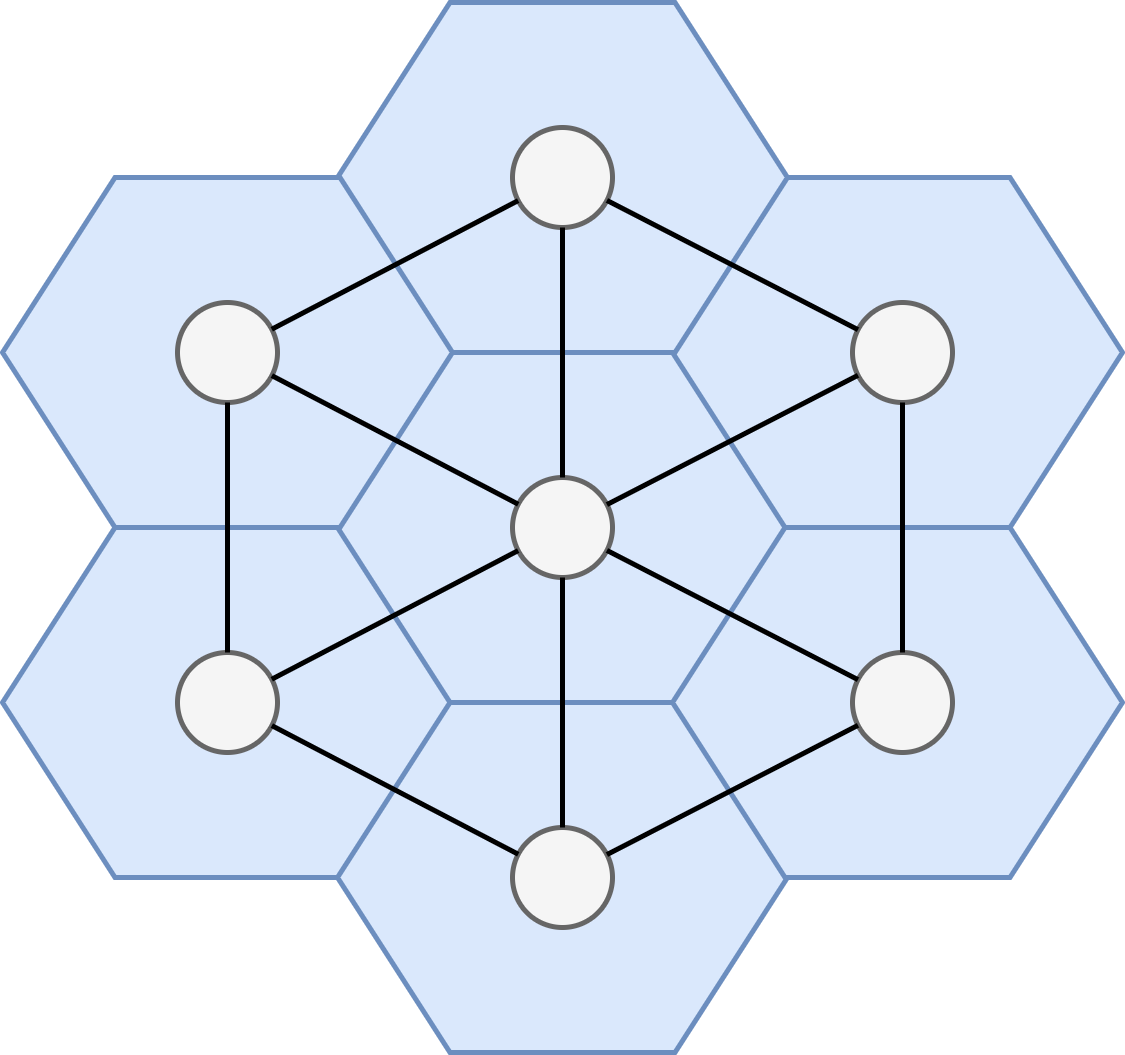
\includegraphics[scale=0.15]{figures/cellular-graph.png}
\caption{An example of a cellular graph}\label{fig:cellular-graph}
\end{figure}
\begin{defin} A cellular network is $k$\textit{-band buffering} if the interference extends up to $k$ cells.
\end{defin}
\begin{defin} Let $G$ be a graph and $L(v)$ a set of colors for all $v \in V(G)$ such that $|L(v)|=k$. We say that $G$ is $k$\textit{-choosable} if $G$ is colorable such that the color of $v$ is in $L(v)$ for all $v \in V(G)$, such colorings called $k$\textit{-list coloring} of $G$.
\end{defin}
\begin{defin} The \textit{choice number} of $G$ is the smallest $k \in \mathbb{N}$ (notated by $\ch(G)$) such that $G$ is $k$-choosable.
\end{defin}
It is worth pointing out that proving a graph to be $k$-choosable is more difficult than showing that it is $k$-colorable. This simply follows from the fact that the lists $L(v):=\lbrace 1,2,3,\ldots,k\rbrace$ for all $v \in V(G)$ bring us back to the original $k$-coloring problem. This observation yields our first bound, that is, $\chi(G) \leqslant \ch(G)$ for any graph $G$. Therefore, it is not surprising that there exists a non $2$-choosable but $2$-colorable graph.
\begin{example}[A non $2$-choosable graph $G$ with $\chi(G)=2$]\label{ex:2-colorable-ch3}
To construct such an example, let us consider the graph in Figure \ref{fig:2-colorable-ch3}. Its coloring immediately shows that $\chi(G)=2$. For the choice number imagine that the numbers inside the nodes correspond to the list of available colors at each node.
\begin{figure}[!h]
\centering
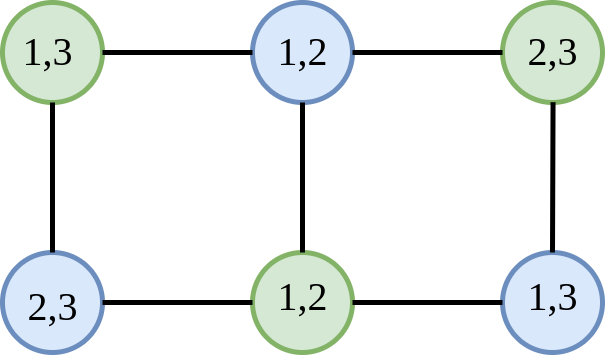
\includegraphics[scale=0.3]{figures/2-colorable-3ch.png}
\caption{A non $2$-choosable graph $G$ with $\chi(G)=2$}\label{fig:2-colorable-ch3}
\end{figure}
Selecting either color $1$ or color $3$ in the upper-left corner leads to a conflict in the coloring and thus $G$ is not $2$-choosable.
\end{example}
\begin{theo}\label{theo:logarithm-bound}
Let $G$ be any graph with $n$ nodes. Then $\ch(G) \leqslant \chi(G) \ln{n}$.
\end{theo}
\begin{proof} To prove the inequality, we use a probabilistic argument. Assume that $G$ is colored with $s := \chi(G)$ colors, that is, the nodes $V(G)$ are divided into the color classes $C_1, C_2, \ldots, C_s$. Suppose that $G$ has a $k$-list assignment $L$ where $k = \chi(G) \ln{n}$ and $n := |V(G)|.$ Consider the probability space of the $s$-partitions $\pi \colon \pi_{1},\pi_{2},\ldots,\pi_{s}$ of $\bigcup_{v \in V(G)} L(v).$ If we can assign for all $i \in \lbrace 1,2,3,\dots,s \rbrace$ a partition $\pi_i$ to the color class $C_i$ such that for all $v \in C_i$ we have $L(v) \cap P_i \neq \varnothing$, then $G$ can be colored from the lists $L$. 

It remains to prove that such a partition $\pi$ exists with nonzero probability and thus the assertion follows. Let us first calculate the probability of the complementary event:
\begin{equation*}
\begin{split}
\mathbb{P}(\exists i \in \lbrace 1,2,\ldots, s \rbrace, \exists v \in C_i, L(v) \cap P_i = \varnothing) = \\
\sum_{v \in V(G)}\left( 1 - \frac{1}{s} \right)^k = n \left(\left(1 - \frac{1}{s} \right)^s \right)^{\frac{k}{s}} < n\mathrm{e}^{-\frac{k}{s}}.
\end{split}
\end{equation*}
The term $\left( 1 - \frac{1}{s} \right)$ is the probability of $c \in L(v)$ not being in $P_i.$ Since there are $k$ colors in each list and we consider every node, the summation is valid. From the equation $k = s \ln{n}$, it follows that $n = \mathrm{e}^{k/s}$ and therefore $n\mathrm{e}^{-k/s} = 1.$ Since the complementary event is not a sure event, it follows that
$$
\mathbb{P}(\forall i \in \lbrace 1,2,\ldots, s \rbrace, \forall v \in C_i, L(v) \cap P_i \neq \varnothing) > 0
$$
which completes the proof.
\end{proof}
\begin{note}From now on we assume that all graphs are connected. We can do it without the loss of generality as all the algorithms and proofs can be repeated for each connected component of a graph.\end{note}

\subsection{Degree bounded acyclic orientations of cellular graphs}\label{sec:orientation}


%%%%%%%%%%%%%%%%%%%%%%%%%%%%%%%%%%%%%%%%%%%%%%%%%%%%%%%%%%%%%%%%%%%%%%%%%%%%%%%%

\begin{lem}\label{lem:degree-constraint}
Let $G$ be a cellular graph. Then $G$ has a node $v$ such that $\deg(v) \leqslant 3$.
\end{lem}

\begin{proof} Let us consider the planar drawing of the graph $G$ which corresponds to its hexagonal topology.
Let $v$ be any node of $G$ and we assign $(0,0)$ to this node. We assign coordinates to every node starting from node $v$ in the following way. If a node $w$ is to the north of node $v$ then the coordinates of node $w$ is equal to the coordinates of node $v$ plus $(0,1)$. We summarize this method in Fig. \ref{fig:assignment} according to the cardinal directions.
\begin{figure}[!h]
\centering
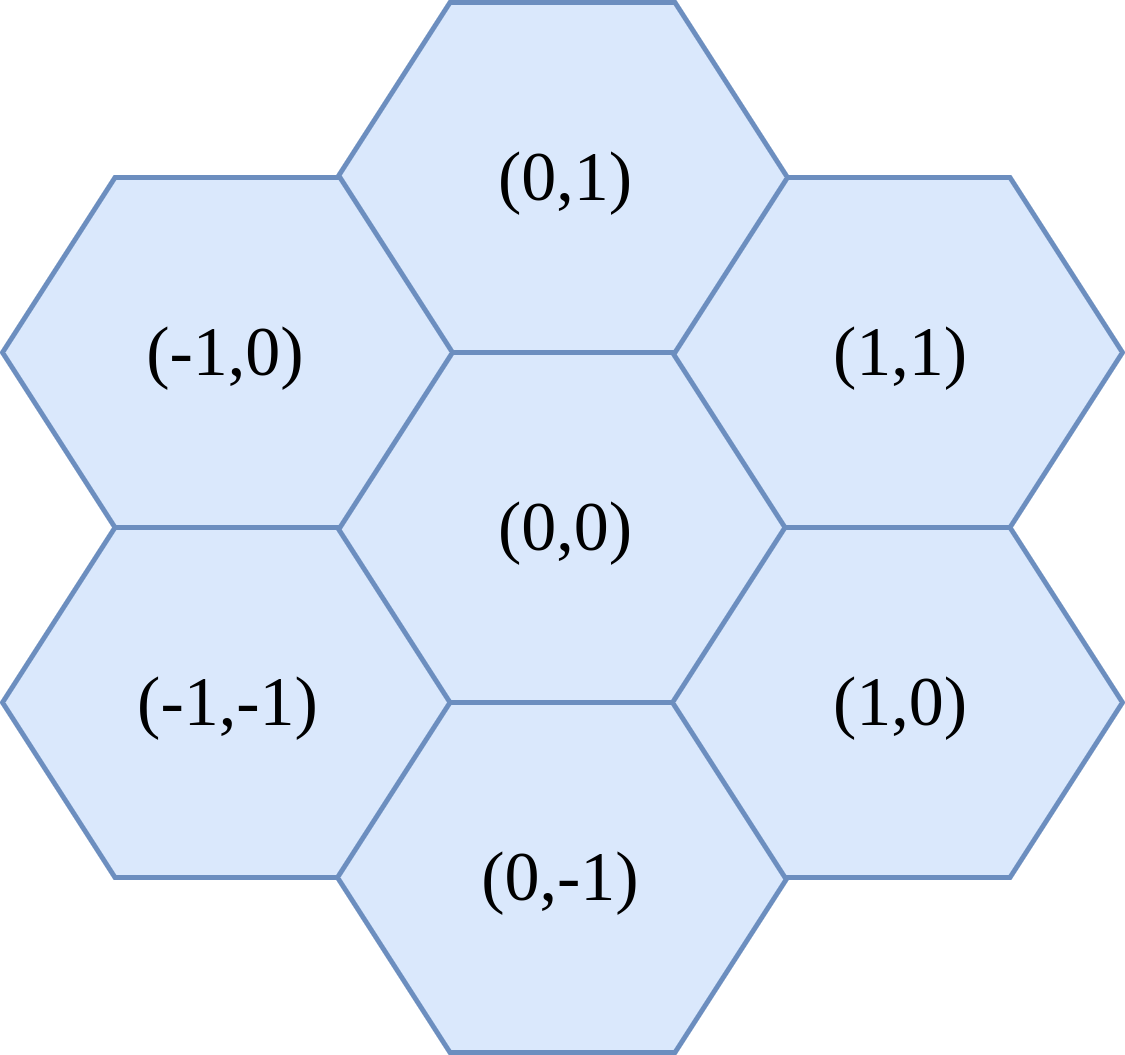
\includegraphics[scale=0.15]{figures/hexagonal-coordinate-system.png}
\caption{Hexagonal coordinate system}\label{fig:assignment}
\end{figure}
By applying this method to every node, we get a coordinate system within our hexagonal topology. Since there are finitely many node in $V(G)$, we can select the maximal node by selecting the node with maximal $x$- and $y$-coordinate, that is, a node $w$ with the following property: if $(x_1,y_1)$ is the coordinates of $w$ and $v \neq w$ is another node with the coordinates $(x_2,y_2)$ then $x_1 \geqslant x_2$ and $y_1 > y_2$ are satisfied.

To obtain a contradiction, suppose that the maximal node $w$ has more than 3 neighbors. It follows then at least one if its neighbors is either to the north, northeast or southeast to $w$. However, this neighbor would violate the maximality of $w$. Therefore we proved that $\deg(w) \leqslant 3$.
\end{proof}
\begin{defin}
We say that the orientation of a digraph $G$ is $k$\textit{-bounded} if for each node $v \in V(G)$ its outdegree is bounded by $k$, that is, $\deg^+(v) \leqslant k$.
\end{defin}
\begin{lem}\label{lem:bounded-acyclic-orientation}
If $G$ is a cellular graph, then $G$ has a $3$-bounded acyclic orientation.
\end{lem}
\begin{proof} Since $G=(V,E)$ is a cellular graph, we can make use of Lemma \ref{lem:degree-constraint}, that is, let $v$ be a node of $G^{(0)}:=G$ with $\deg(v) \leqslant 3$. We construct a function $f\colon V(G) \to \mathbb{N}$ by setting $f(v) := 0$ and then remove the node $v$ from $G^{(0)}$ yielding the graph $G^{(1)}$. By repeating the same procedure\---at step $i$th\---we select a node $v$ in $G^{(i)}$ such that $\deg(v) \leqslant 3$ and we set $f(v):=i$. Then we remove $v$ from $G^{(i)}$ which yields the graph $V(G^{(i+1)}) := V(G^{(i)}) \setminus \lbrace v \rbrace$. It is trivial that the graphs $G^{(1)},\ldots,G^{(|V(G)|)}$ are all cellular therefore it was valid using Lemma \ref{lem:degree-constraint}.

We note that the procedure ends after $|V(G)|$ steps.

Now we construct a digraph $H=(V,A)$ from $G$ using the function $f$. Let $(u,v) \in E$ be an arbitrary edge. If $f(u) < f(v)$ then $A:=A\cup (u,v)$ otherwise $A:=A \cup (v,u)$. By repeating this procedure for all edges in $E$ we get an orientation of $G$, that is, the digraph $H$. We need to prove that $H$ is
\begin{enumerate}
\item acyclic and
\item $\deg^+(v) \leqslant 3$ holds for all $v \in V(G)$.
\end{enumerate}
To prove (1), we will obtain a contradiction by assuming that $H$ contains a directed cycle. Let $C$ be a directed cycle in $H$ with the nodes $C:=\lbrace v_1,v_2,\ldots,v_k \rbrace$ that are ordered such that $(v_i,v_{i+1 \bmod{k}}) \in E$ $(i=1,2,\ldots,k)$ which means that $f(v_1) < f(v_2) < \ldots < f(v_{k-1}) < f(v_k)$ but also $f(v_k) < f(v_1)$ which is impossible.

What is left to show is that $\deg^+(v) \leqslant 3$. At each step we select a node with no more than $3$ neighbors and those neighbors will be assigned a number that is greater than $f(v)$. Therefore the outdegree of $v$ cannot be larger than $3$.
\end{proof}

It is easy to see that the proof of this lemma can be transformed into a polynomial time algorithm. We outline the algorithm (Algorithm \ref{alg:find-acyclic-bounded-orientation}) that is based on the proof of Lemma \ref{lem:bounded-acyclic-orientation} and then we prove that its running time is $O(|V(G)| + |E(G)|)$.
\begin{algorithm}\label{alg:find-acyclic-bounded-orientation}
 \KwData{A cellular graph $G = (V,E)$}
 \KwResult{An acyclic $3$-bounded orientation of $G$}
 $G^{(0)} := G$\;
 Initialize $f \colon V(G) \to \mathbb{N}$\;
 \For{$i\leftarrow 0$ \KwTo $|V(G)|-1$}{
  Select $v \in V(G^i)$ such that $\deg(v) \leqslant 3$\;
  $f(v):=i$\;
  $V(G^{(i+1)}):=V(G^{i}) \setminus \lbrace v \rbrace$\;
 }
 Initialize $H:=(V,A)$\;
 \ForAll{$e = (u,v) \in E(G)$}{
   \eIf{$f(u) < f(v)$} {
   	$A := A \cup (u,v)$\;
   }{
   $A := A \cup (v,u)$\;
   }   
 }
 \caption{Constructing an $3$-bounded acyclic orientation of a cellular graph}
\end{algorithm}
\begin{state}\label{state:acyclic-complexity-proof} Algorithm \ref{alg:find-acyclic-bounded-orientation} has a running time of $O(|V(G)| + |E(G)|)$.
\end{state}
\begin{proof}
It is enough to prove that "Select $v \in V(G^i)$ such that $\deg(v) \leqslant 3$" can be done in $O(|V(G)|)$ since the rest is obvious. Let us initialize a queue $Q := \lbrace v \mid \deg(v) \leqslant  3\rbrace$ before we start running the algorithm. We pop a node $v$ from $G$ at every iteration and push new ones after the removal of $v$ if there are new nodes in $G$ that satisfy the degree condition. The pop and push methods can be implemented in constant time which completes the proof.
\end{proof}

\begin{note} We would like to note that a more general proposition can be formulated from Lemma \ref{lem:bounded-acyclic-orientation} without assuming that $G$ is cellular. If we can ensure that in each step a node $v$ with $\deg(v) \leqslant k$ can be selected then the algorithm will yield a $k$-bounded acyclic orientation in arbitrary graphs.
\end{note}

\begin{defin} We say that the Szekeres\---Wilf number of a graph $G$ is $k$ if every subgraph of $G$ contains a node of degree at most $k$. The term $k$-degeneracy is also used in some literature.
\end{defin}

Immediately follows that if we omit the cellular graph assumption\---having known that the Szekeres\---Wilf number of graph is $k$\---then the arguments of the proof of Lemma \ref{lem:bounded-acyclic-orientation} can be repeated and thus the following lemma holds.

\begin{lem}\label{lem:szekeres} Let $G$ be any graph such that its Szekeres\---Wilf number is $k$. Then $G$ has a $k$-bounded acyclic orientation. \qed
\end{lem}

Another interesting question is how to compute the Szekeres\---Wilf number of a graph. The following algorithm \cite{Matula:1983:SOC:2402.322385} computes this number in linear time by repeatedly removing the minimum-degree nodes.

\begin{algorithm}\label{alg:szekeres-wilf-computation}
 \KwData{An arbitrary graph $G = (V,E)$}
 \KwResult{The Szekeres\---Wilf number of $G$ in $szw$}
 $H^{(1)} := G$\;
 $szw := 0$\;
 \For{$i\leftarrow 1$ \KwTo $|V(G)|$}{
  Select $v_i \in V(H^{i})$ such that $\deg(v) = \delta(G)$\;
  $szw := \max(\deg(v_i), szw)$\;
  $V(H^{i+1}) := V(H^{i}) \setminus \lbrace v \rbrace$\;
 }
 \caption{Computing the Szekeres\---Wilf number of an arbitrary graph}
\end{algorithm}
\begin{proof}
The linear time is obvious as we iterate through the nodes of $G$. The efficient selection of the minimum-degree node is described in the proof of Proposition \ref{state:acyclic-complexity-proof}. Let $k$ be the Szekeres\---Wilf number of $G$. It is obvious that $szw \leqslant k = \max_{H \subset G} \delta(H)$. To obtain a contradiction assume that $szw < k$. Now let $H$ be the "maximal" subgraph in $G$, that is, $szw < \delta(H) = k$. Let $i$ be the smallest index such that $v_i \in V(H)$. Due to our choice we have $H \subset H_i$. Then $\deg_{H_i}(v_i) = \delta(H_i) \leqslant szw < k = \delta(H) \leqslant \deg_H(v_i)$. However, from $H \subset H_i$, it follows that $\deg_H(v_i) \leqslant \deg_{H_i}(v_i)$ which is a contradiction and therefore $k = szw$ as required.
\end{proof}

\subsection{Defective coloring}\label{sec:defective}
In some cases, it is impossible to assign the channels such that the allocation yields an interference-free system. 
\begin{defin} We say that a graph $G$ is $(k,d)$-colorable if the graph can be colored with $k$ colors such that every color class induces a graph with maximum degree at most $d$.
\end{defin}

Such colorings are known as \textit{defective} or \textit{improper} coloring since the definition allows the nodes to have at most $d$ neighbors from the same color class.
A classical result from Lovász shows that an arbitrary graph can be colored with $k$ colors in polynomial time with at most $[\Delta(G)/k]$ ''errors''.
\begin{theo}[Lovász]\label{theo:lovasz-defective}
Let $G$ be any graph and $k > 0$ then $G=(V,E)$ is $(k,[\Delta(G)/k])$-colorable in $O(|E|)$ steps.
\end{theo}
\begin{proof} Let us consider an arbitrary (not necessarily proper) $k$-coloring of $G$. If this coloring is a $(k,[\Delta(G)/k])$-coloring then we are done otherwise choose a node $v$ that has more than $[\Delta(G)/k]$ neighbors from the same color class. It is obvious that there exists a color class $c$ with at most $[\Delta(G)/k]$ nodes in the neighbor set of $v$. By changing the color class of $v$ to color class $c$, we decrease the monochromatic edges in the coloring by at least one. Therefore we reach a $(k,[\Delta(G)/k])$-coloring in at most $|E|$ steps.
\end{proof}

\paragraph*{References} Example \ref{ex:2-colorable-ch3} is from \cite{erdos-choosability} \textit{Example scheme showing how choice $\ch(G)$ exceeds $\chi(G)$}. The proof of Theorem \ref{theo:logarithm-bound} can be found at \url{http://www.math.uri.edu/~eaton/TalkUriOct03P2.pdf} (accessed on the 9th March 2018). The idea of Algorithm \ref{alg:find-acyclic-bounded-orientation} came from \cite{CHROBAK1991243} \textit{Theorem 2.1} where the authors proved that every planar graph has a $5$-bounded acyclic orientation. They used the fact that every planar graph has a node with at most $5$ neighbors which follows from Euler's formula. Theorem \ref{theo:lovasz-defective} is from \cite{Cowen:1997:CD:314161.314387} \textit{Theorem 1.1} and the proof of Algorithm \ref{alg:szekeres-wilf-computation} can be found in \cite{Matula:1983:SOC:2402.322385} \textit{2. Smallest-Last Vertex Ordering}.

\section{$1$-band buffering cellular graphs are $4$-choosable}\label{sec:4-choosable}
We are about to prove one of our main results, that is, cellular graphs are $4$-choosable. We would like to note that since $G$ is a planar, it follows from Thomassen's theorem \cite{Thomassen:1994:PG:184180.184192} that it is $5$-choosable. It is worth noting that cellular graphs are $3$-colorable \cite{662943} (Theorem 1). However, even with this additional constraint, we still cannot say that if $G$ is planar and $3$-colorable then it is $4$-choosable as a counterexample can be found in \cite{JGT:JGT4}. The counterexample is quite interesting (\cite {JGT:JGT4}, second figure) as it is constructed from a cellular graph; however the author added one extra node and joined it to all of the outer nodes. Due to this step, the resulting graph does not always contain a node of degree $3$ therefore the property of Lemma \ref{lem:degree-constraint} is not true for this construction.

In Section \ref{sec:kernel-perf-and-galvin} we introduce the notion of kernel, kernel-perfectness and Galvin's theorem which gives a sufficient condition for being $k$-choosable. Section \ref{sec:dag} details the fast computation of kernels in DAGs. Finally, a polynomial time algorithm that 4-list colors an arbitrary cellular graph is given in Section \ref{sec:4-list-coloring}.
\subsection{Kernel-perfectness and theorem of Galvin}\label{sec:kernel-perf-and-galvin}
Before proving our theorem we need to introduce the notion of kernel in graphs and a theorem from Galvin \cite{Galvin:1995:LCI:199352.199369} (non-multigraph version from \cite{citeulike:395714}, Lemma 5.4.3) that will play a central role in our study. The proof of the theorem is inductive and can be transformed into an algorithm.
\begin{defin} Let $G$ be a directed graph. We say that an independent set $K \subseteq V(G)$ is a kernel of $G$ if it satisfies the following: for each node $u \in V(G) \setminus K$ there is a node $v \in K$ such that $(u,v) \in E(G)$.
\end{defin}
\begin{theo}[Galvin, 1995]\label{thm:galvin} Let $G$ be a graph and $\lbrace L(v) \mid v \in V(G) \rbrace$ given color sets. If $G$ has an orientation $D$ such that $d^+(v) < |L(v)|$ for all $v \in V(D)$ and every induced subgraph of $D$ has a kernel, then $G$ can be colored from the given color sets. $\blacksquare$
\end{theo}
We postpone giving a proof of this theorem as we will reformulate Galvin's theorem for cellular graphs later.
\begin{defin} We note that a directed graph is called kernel-perfect if all of its induced subgraphs contain a kernel.
\end{defin}
\begin{theo}\label{thm:choice-number}
If $G$ is a cellular graph then $\ch(G) \leqslant 4$.
\end{theo}
\begin{proof}
Since $G$ is cellular, we can consider its $3$-bounded acyclic orientation by Lemma \ref{lem:bounded-acyclic-orientation}. This orientation is kernel-perfect by Richardson's theorem \cite{richardson1946}. Therefore we can apply Theorem \ref{thm:galvin} (with $d^+(v) \leqslant 3$ and $L(v)=4$) which concludes the proof.
\end{proof}

We have proven that cellular graphs are $4$-choosable, hence what is left is to show that there exists an algorithm that constructs such colorings in polynomial time.
\subsection{Finding a kernel in DAGs}\label{sec:dag}

It has been shown that finding a kernel in an arbitrary graph is $\mathrm{NP}$-complete \cite{chvatal}. However, we will show that in directed acyclic graphs (DAGs) this problem can be easily solved in polynomial time. This is crucial as our $4$-list coloring algorithm has to construct kernels repeatedly at run.

\begin{lem}\label{lem:kernel-lemma} Let $G$ be a directed acyclic graph. Then a kernel $K \subseteq V(G)$ can be found in polynomial time.
\end{lem}
\begin{proof} Since $G$ is acyclic we can consider the topological order of its nodes (which can be computed in polynomial time). Let $\lbrace v_1, v_2, \ldots, v_n \rbrace$ be this topological order. Let us start from node $v_n$ and add it to the kernel, that is, $K = \lbrace v_n \rbrace$. Mark the neighbors of $v_n$. After that, we move on with the next node $v_{n-1}$, if it is marked we skip it otherwise we add it to the kernel $(K := K \cup \lbrace v_{n-1} \rbrace)$ and mark its neighbors. Repeat this procedure with the remaining nodes. We need to prove that
\begin{enumerate}
\item $K$ is independent and
\item for each node $u \in V(G) \setminus K$ there is a node $v \in K$ such that $(u,v) \in E(G)$.
\end{enumerate}
1) If $v \in K$ then its neighbors are marked. Since we do not add marked nodes to $K$, it is always independent.
2) When $v$ is unmarked and we add it to $K$ all of its neighbors come after it in the topological order (otherwise $v$ would have already been marked), that is, $v$ is connected to its neighbors by forward edges.
\end{proof}
\begin{algorithm}\label{alg:find-kernel-in-dags}
 \KwData{A directed acyclic graph $G = (V,A)$}
 \KwResult{A kernel $K \subseteq V(G)$}
 $T := \text{the topological order of $V(G)$}$\;
 $K := \emptyset$\;
 \For{$i\leftarrow |V(G)|$ \KwTo $1$}{
  \If{$T(i)$ is unmarked} {
  	$K := K \cup \lbrace T(i) \rbrace$\;
  	Mark the neighbors of $T(i)$\;
  }
 }
 \caption{Finding a kernel in a DAG}
\end{algorithm}

We note that the topological order can be computed in linear time in the number of nodes and edges with Kahn's algorithm \cite{Kahn:1962:TSL:368996.369025}, therefore the running time of our algorithm is $O(|V(G)|+|E(G)|)$. We also note that an induced subgraph of a DAG is trivially a DAG, therefore from Algorithm \ref{alg:find-kernel-in-dags} it follows that DAGs are kernel-perfect, that is, there is no need to apply Richardson's theorem in the proof of Theorem \ref{thm:choice-number}. 

Finally, it is worth mentioning that Von Neumann and Morgenstern \cite{neumann} proved that the kernel of a DAG is unique, that is, the output of Algorithm \ref{alg:find-kernel-in-dags} is independent of the selected topological order.
\subsection{$4$-list coloring of cellular graphs}\label{sec:4-list-coloring}
Now we have everything necessary to prove our main result and give a polynomial algorithm that computes a $4$-list coloring of a cellular graph. 

First, we reformulate Galvin's theorem for cellular graphs and prove it (Theorem \ref{thm:galvin}), the proof is based on \cite{citeulike:395714} (Lemma 5.4.3). The original proof uses mathematical induction, we just repeat the same argument, fortunately, the inductive step describes how to color the nodes, that is, the proof can be transformed into an algorithm. The cellular version, however, uses our result, namely Lemma \ref{lem:bounded-acyclic-orientation}. In addition, it also uses Lemma \ref{lem:kernel-lemma}. Then we prove that its (Algorithm \ref{alg:four-list-coloring}) running time is polynomial. Algorithm \ref{alg:four-list-coloring} uses Algorithm \ref{alg:find-acyclic-bounded-orientation} and Algorithm \ref{alg:find-kernel-in-dags}. The fact that Algorithm \ref{alg:four-list-coloring} is polynomial follows from the fact that Algorithm \ref{alg:find-acyclic-bounded-orientation} and Algorithm \ref{alg:find-kernel-in-dags} are polynomial.
\begin{theo}[Galvin's theorem for cellular graphs] Let $G$ be a graph and $\lbrace L(v) \mid v \in V(G) \rbrace$ given color sets. If $G$ has a kernel-perfect orientation $D$ such that $d^+(v) < |L(v)|$ for all $v \in V(D)$, then $G$ can be colored from the given color sets.
In particular, if $G$ is a cellular graph and $|L(v)| \geqslant 4$ for all $v \in V(G)$. Then $G$ can be colored from the given color sets.
\end{theo}
\begin{proof}
Let $G^*$ be the $3$-bounded acyclic orientation of $G$ (Lemma \ref{lem:bounded-acyclic-orientation}), that is, $d^+(v) \leqslant 3$. We apply induction on $|V(G^*)|$. For $|V(G^*)|=0$, the empty coloring is good. Let us assume that we know how to color $G^*$ with $|V(G^*)| < n$ and consider the case when $|V(G^*)|=n$. Let $\alpha$ be any color from one of the colors sets and set $V_\alpha$ to $\lbrace v \in V(G) \mid \alpha \in L(v) \rbrace$. Consider the non-empty subgraph $D$ of $G^*$ that is spanned by $V_\alpha$. Since $G^*$ is a DAG, it is kernel-perfect (Lemma \ref{lem:kernel-lemma}), therefore $D$ has a kernel $U \neq \emptyset$. Assign the color $\alpha$ to every node in $U$ and remove $\alpha$ from $L(v)$ for all $v \in V_\alpha$. Since $U$ is independent, and we removed $\alpha$, it follows that we did not (and we will not) violate the rules of the graph coloring. After that, remove $U$ from $D$, since every node in $V(D) \setminus U$ sends an edge to $U$, having removed $U$ from $D$, we decreased the outdegree of each node in $D$ by $1$. Since the modified lists $L'(v)$ $(v \in V_\alpha)$ satisfy $d^+(v) < |L'(v)|$ for all $v \in V(D) \setminus U$, we can use our induction hypothesis to color $V(G^*) \setminus U$.
\end{proof}
\begin{algorithm}\label{alg:four-list-coloring}
 \KwData{A cellular graph $G$ and a set of colors $L(v)$ for all $v \in V(G)$ with $|L(v)| \geqslant 4$}
 \KwResult{$4$-list coloring of $G$}
  Let $G^*$ be the $3$-bounded acyclic orientation of $G$ (Algorithm \ref{alg:find-acyclic-bounded-orientation})\;
  \While{$V(G^*)$ is non-empty} {
  	Let $\alpha$ be a color from $L(v)$ where $v \in V(G^*)$\;
  	$V_\alpha := \lbrace v \in V(G) \mid \alpha \in L(v) \rbrace$\;
  	Let $D$ be the subgraph of $G^*$ that $V_\alpha$ spans\;
  	Let $U$ be a kernel in $D$ (Algorithm \ref{alg:find-kernel-in-dags})\;
  	Color the nodes in $U$ with color $\alpha$\;
  	Remove $\alpha$ from $L(v)$ for all $v \in V_\alpha$\;
  	Remove the colored nodes, that is, $V(G^*) := V(G^*) \setminus U$\;
  }
 \caption{$4$-list coloring of a cellular graph}
\end{algorithm}

It can be seen from the algorithm that first we call Algorithm \ref{alg:find-acyclic-bounded-orientation} then we call Algorithm \ref{alg:find-kernel-in-dags} multiple times. If we assume the worst-case scenario when the kernel $U$ has only $1$ element, then the while loop iterates $|V(G)|$ times. The auxiliary operations such as spanning a subgraph or creating the set $V_\alpha$ can be done in linear time. Therefore the overall running time of our algorithm is $O(|V(G)|^2+|V(G)||E(G)|)$.

In each iteration, we color the nodes in $U$ and remove one color. The color is proper by Theorem \ref{alg:four-list-coloring}. However, we need to show that in each iteration every node is either colored or it has a free available color.
\begin{lem} Algorithm \ref{alg:four-list-coloring} is correct, that is, in each iteration every node is either colored or it has a free available color.
\end{lem}
\begin{proof} To obtain a contradiction, let us suppose that there is a node $v$ that is not colored and it does not have an available color ($|L(v)|=0$). This means that $v$ was in $V_{\alpha}$ for at least $4$ different colors and it was never in the kernel. However, this would mean that $d^+(v) \geqslant 4$ as $v$ sent an edge to each kernel. This is impossible since $G$ is $3$-bounded.
\end{proof}

\paragraph*{References} Galvin's theorem with proof can be found in \cite{citeulike:395714} \textit{Lemma 5.4.3}.

\section{The $k$-band buffering case}
In this section, we generalize the current results for $k > 1$. From Galvin's theorem and Lemma \ref{lem:szekeres}, it can be seen that a graph is $(k+1)$-choosable if $G$ has a Szekeres\---Wilf number of $k$, in other words if $G$ has a $k$-bounded acyclic orientation then it is $(k+1)$-choosable.

By exploiting the special structure of $1$-band buffering cellular graphs, we found that such graphs always have a node with $\deg(v) \leqslant 3$ (Lemma \ref{lem:degree-constraint}). Lemma \ref{lem:bounded-acyclic-orientation} used this property to prove that they admit a $3$-bounded acyclic orientation.

Even though Algorithm \ref{alg:four-list-coloring} is designed for $1$-band buffering cellular graphs, the input graph $G$ can be easily modified such that running Algorithm \ref{alg:four-list-coloring} properly $l$-list-colors $G$ while it does not violate the $k$-band buffering requirement. The usual trick to do this is to construct a graph $G'$ from $G$ such that $V(G') := V(G)$ and
$$(u,v) \in E(G') \text{ if and only if } d_{G}(u,v) \leqslant k$$
where $d_{G}(u,v)$ is the distance between $u$ and $v$ in $G$, that is, the length of the shortest path that connects $u$ and $v$. It is trivial that running Algorithm \ref{alg:four-list-coloring} for $G'$ is equivalent to running a $k$-band buffering list-coloring algorithm  for $G$.

Obviously, we also need to modify Algorithm \ref{alg:find-acyclic-bounded-orientation} as we do not know the Szekeres\---Wilf number of $G'$. Algorithm \ref{alg:find-acyclic-bounded-orientation-general} simply modifies Algorithm \ref{alg:find-acyclic-bounded-orientation} by selecting a node with $\deg(v) = \delta(G^i)$ in each iteration $i$ which is the same step that Algorithm \ref{alg:szekeres-wilf-computation} carries out to compute the Szekeres\---Wilf number. Therefore the following theorem holds:

\begin{theo} Algorithm \ref{alg:find-acyclic-bounded-orientation-general} computes an $l$-bounded acyclic orientation of an arbitrary graph $G$ where $l$ is the Szekeres\---Wilf number of $G$.
\end{theo}

\begin{proof} Immediately follows from Algorithm \ref{alg:find-acyclic-bounded-orientation} and \ref{alg:szekeres-wilf-computation}.
\end{proof}

\begin{algorithm}\label{alg:find-acyclic-bounded-orientation-general}
 \KwData{A cellular graph $G = (V,E)$}
 \KwResult{An acyclic $l$-bounded orientation of $G$}
 $G^{(0)} := G$\;
 Initialize $f \colon V(G) \to \mathbb{N}$\;
 \For{$i\leftarrow 0$ \KwTo $|V(G)|-1$}{
  Select $v \in V(G^i)$ such that $\deg(v) = \delta(G^i)$\;
  $f(v):=i$\;
  $V(G^{(i+1)}):=V(G^{i}) \setminus \lbrace v \rbrace$\;
 }
 Initialize $H:=(V,A)$\;
 \ForAll{$e = (u,v) \in E(G)$}{
   \eIf{$f(u) < f(v)$} {
   	$A := A \cup (u,v)$\;
   }{
   $A := A \cup (v,u)$\;
   }   
 }
 \caption{Constructing an $l$-bounded acyclic orientation of a $k$-bounded cellular graph where $l$ is the Szekeres\---Wilf number of $G$}
\end{algorithm}

The following question immediately arises: how large is the Szekeres\---Wilf number of $k$-band buffering cellular graphs? Unfortunately, we cannot answer this question, however the following theorem gives us an upper bound and as a corollary it turns out that $k$-band buffering cellular graphs are $(3(k+1)k/2+1)$-choosable.

\begin{theo} Let $G$ be a $k$-band buffering cellular graph then $G$ has a node with $\deg(v) \leqslant 3(k+1)k/2$.
\end{theo}
\begin{proof}
\end{proof}
\section{Local graph algorithms for list coloring}

\subsection{The local model}

\newpage
\printbibliography
\addcontentsline{toc}{section}{References}
\end{document}
